\documentclass[a4paper,11pt]{article}
\usepackage{graphicx} % Required for inserting images
\usepackage[margin=1in]{geometry}
\usepackage{enumerate,setspace}
\usepackage{amsmath}
\usepackage{tabularx,array,booktabs,caption}
\usepackage[hidelinks]{hyperref}
\usepackage{fancyhdr}
\usepackage{titlesec}
\usepackage{setspace} 
\usepackage{indentfirst} 
\usepackage[style=apa]{biblatex}
\usepackage{float}
\usepackage{subcaption} 
\usepackage{longtable}
\usepackage{hyperref}
\usepackage{algorithm}
\usepackage{algpseudocode}
\usepackage{enumitem}
\usepackage{booktabs}
\usepackage{siunitx}
\usepackage{multirow}
\usepackage[utf8]{inputenc}
\usepackage{tikz}
\usetikzlibrary{shapes.geometric, arrows.meta, positioning, calc}

\usepackage{caption}
\usepackage[font=it]{caption}
\usepackage[justification=raggedright,singlelinecheck=false]{caption}
\captionsetup[table]{justification=raggedright, singlelinecheck=false}

\addbibresource{references.bib}

% change font style to ariel
\usepackage{helvet}
\renewcommand{\familydefault}{\sfdefault}



\begin{document}

\begin{titlepage}
    \onehalfspacing
    \normalsize
    \renewcommand{\familydefault}{\sfdefault}
    \begin{center}
        {\Huge Comparison of Numerical Iterative Methods in Solving Eccentric Anomalies In Kepler's Equation For Orbital Motion}\\
        \vspace{48pt}
        {\bfseries BSM Computer Science - CS 4A}\\
        Manansala, Richard M.\\
        Dalugdugan, Nicko\\
        Delos Santos, Melchor\\
        Nicolas, John Clarence\\
        \vspace{48pt}
        College of Science\\
        Mathematics Department\\
        March 2026\\
        A.Y. 2025-2026, 2nd Semester
    \end{center}
    \newpage
    \begin{abstract}
    \onehalfspacing
    \normalsize

\end{abstract}
    \thispagestyle{empty}
    \tableofcontents
    \listoftables
    \thispagestyle{empty}
    \listoffigures
\end{titlepage}


\pagestyle{fancy}
\fancyhf[]{} % Clear all header and footer fields

\fancyfoot[R]{\thepage}
\fancyhead[L]{Comparison of Numerical Iterative Methods in Solving Eccentric Anomalies In Kepler's Equation For Orbital Motion}
\onehalfspacing

\setcounter{page}{1} % Reset the page counter to 1

\section{Introduction}

For centuries, early astronomers believed that the Earth is the center of the universe, and that other planets revolved around it. The geocentric model, or the Ptolemaic system, is an astronomical concept that believes that Earth is the center of the universe, and that stars such as the Sun, Moon, and other planets revolve around it in circular orbits \parencite{sheposh2023geocentric}. This geocentric view was established by a Greek astronomer named Claudies Ptolemaeus in the second century, and would dominate scientific thought due to its alignment with religious beliefs until the arrival of Nicolaus Copernicus, which introduced a heliocentric model back in the sixteenth century. Copernicus  proposed that the Sun, not the Earth, was the center of the Solar System     \parencite{rochesterCopernican}. This model was called heliocentric, as the Earth is just another planet outward from the sun, and the Moon is the one that orbits the Earth, not the sun.

In addition, there's also a prevailing view that thez celestial bodies around us moved in perfect circles, not until the early 17th century that Johannes Kepler, a German astronomer and a mathematician, proved that the planetary orbits do not move in perfect circles, but rather, in ellipses. According to \textcite{berkley2023planetary}, planetary orbits are the paths that planets follow as they travel around the Sun, defined as elliptical shapes rather than perfect circles. Furthermore, the role of gravity influences the speed of the orbiting planets based on their distance from the Sun, and that these planets move faster when they are closer, while the farthest planets move slower.

These observations were not made possible by Kepler alone, but with the help of Tycho Brahe, a Danish astronomer, who provided decades of precise observational data of the stars and the planets. With the help of Brahe's meticulous planetary observations, Kepler was able to form his findings into three fundamental principles, now famously known as the Kepler's Laws of Planetary Motion. The first law, which is the law of ellipses, the second law, which is the law of equal areas, and the third law, which is the law of harmonies. National Aeronautics and Space Administration or \textcite{nasa2024orbits} said that in Kepler's first law, each planet's orbit about the Sun is an ellipse, and that the planets follows the ellipse in its orbit, and these planets constantly change their distance to Sun as they go around their orbit. In the second law, the imaginary line joining a planet and the Sun sweeps equal areas of space during equal time intervals as the planet orbits, which means that the planets' speed varies, where a planet is moving fastest when it's near or at perihelion, while it is slowest when it's at aphelion, or the farthest. Lastly, the third law of Kepler mentioned that  the squares of the orbital periods of the planets are directly proportional to the cubes of the semi-major axes of their orbits, meaning, the farther a planet from the sun, the longer it takes to orbit, the reason why Mercury has 88 days to orbit the sun, while the Earth has 365, and the other planet having different days to orbit.

Although Kepler managed to describe the planetary orbits and the rules of their motion, these laws do not determine the exact position of a planet along that ellipse at any given moment in time. As stated in the second law, a planet's speed constantly changes as it travels its elliptical path, knowing the precise location is complex to solve. To mathematically calculate a planet's exact position on its elliptical path, astronomers use a paramer known as the eccentric anomaly. As explained by \textcite{weisstein2026eccentric}, eccentric anomaly is the angle obtained by drawing the auxiliary circle of an ellipse The angle obtained by drawing the auxiliary circle of an ellipse with center O and focus F, and drawing a line perpendicular to the semimajor axis and intersecting it at A. In simpler terms, an eccentric anomaly helps determine the position of a planet or a celestial body along their elliptical orbit.

Ultimately, the importance and significance of Kepler's discovery with the planetary laws revolutionized the understanding and perspective of humanity with the celestial bodies. Up until today, these principles still remain intact and a foundation for modern astrodynamics and celestial mechanics, as they're actively used by different space agencies and networks to navigate the vast and unknown space, the trajectories of asteroids near the earth, and employing satellites in space. With the study, comparison of different numerical iterative methods helps identify which methods provide the most accurate, and efficient solution for determining the orbiting bodies. In addition to that, the study contributes to the computational techniques used in modern astronomy, as accurate and efficient solutions are essential to bridge classical astronomical theories with modern computational methods to enhance and betterment the understanding of orbital motion.

\subsection{Scope and Limitations}

The primary focus of the study is the comparison of only two iterative root finding methods which are Newton-Raphson and Halley's method in solving the eccentric anomaly in Keppler's first law. The study only compared both methods on three primary metrics: convergence rate or the number of iterations required to find the root, computational efficiency or the average execution time to find the root in microseconds, and stability or the standard deviation of the execution time. Simple additive weighting was also used for the ranking and scoring of the both in the mentioned criterias. The study also adapted the four initial values from the study of Ozuomba as test cases. Python programming language was used for the implementation of both numerical methods as well as their scoring.
The study focused exclusively on high-eccentricity orbital configurations to simulate extreme convergence situations, thereby, excluding other eccentric configurations. The study's numerical methods were executed in a household computer, meaning the results of the study do not account for specific hardware limitations. Each SAW criteria was also given equal weights which assumed equal priority. 

\subsection{Research Questions}

	The primary objective of this study is to perform an analysis and comparison of the iterative root finding methods, Newton-Raphson method and Halley's method in solving for the eccentric anomaly in Keppler's first law. 

The study specifically aims to answer the following:
\begin{enumerate}
    \item How do Newton-Raphson and Halley's methods compare in terms of their convergence rate and computational efficiency when solving Kepler's Equation?
    \item How does the initial guess ($E_0$) influence the stability and convergence speed of these two methods?
    \item Between Newton-Raphson and Halley's methods, which offers the optimal balance of speed, mathematical efficiency, and reliability as determined by the Simple Additive Weighting (SAW) score?
\end{enumerate}


\section{Preliminaries}

\subsection{Orbital Mechanics and Kepler's Equation}

Orbital mechanics is the study of the motion of celestial objects under the influence of gravitational force. The motion of the planets and satellites is generally explained by Kepler's laws of planetary motion. Kepler's laws were derived by Johannes Kepler based on the observations of Tycho Brahe. According to Kepler's first law, the path of the motion of the planets is elliptical with the sun at one of the focuses. The second law of Kepler's states that the line joining the sun to the planet sweeps out an equal area in an equal time. The third law of Kepler's establishes a relationship between the period of the orbit and the semi-major axis of the orbit, expressed as $T^2 \propto a^3$. These principles form the foundation of classical orbital mechanics and are widely used in astronomy, astrophysics, and satellite motion analysis \parencite{salah2025kepler}.

To determine the position of a body in an elliptical orbit at a specified time, the field of orbital mechanics has proposed angular parameters called anomalies, which include the mean anomaly, eccentric anomaly, and true anomaly. The relationship between the mean anomaly $M$, eccentric anomaly $E$, and orbital eccentricity $e$ is given by Kepler's Equation

\begin{equation*}
M = E - e \sin E
\end{equation*}

\noindent where $0 \leq e \le 1$ represents the eccentricity of the orbit.

The equation is a transcendental equation because the variable E appears both algebraically and trigonometrically. This means that the equation cannot be solved algebraically, but numerical methods must be used to find the value of the eccentric anomaly E. This is done by rearranging the equation
\begin{equation*}
    E - e \sin E - M = 0
\end{equation*}
In this regard, the problem becomes a nonlinear root-finding problem that can be addressed using various iterative numerical methods such as fixed-point iteration, Newton's method, and Halley's method. These numerical methods can be employed in orbital computations for obtaining accurate approximations for the eccentric anomaly \parencite{salah2025kepler}.
 
\subsection{Numerical Root-Finding Algorithms}

\subsubsection{Newton-Raphson Method}

\subsubsection{Halley's Method}

\subsection{ Multi-Criteria Decision Making \& Simple Additive Weighting}

\section{Methods and Applications}

The Keppler's First law relates the mean anomaly, M, and the eccentric anomaly, E, as follows:
\begin{equation*}
M = E - e \sin E
\end{equation*}

With that, the function to approximately find the root with the numerical methods is as follows:
	\begin{equation*}
        f(E) = E - e \sin E - M
    \end{equation*}
Where $E$ is the eccentric anomaly, $M$ is the mean anomaly, and $e$ is the eccentricity of the orbit.

\subsection{Newton Raphson Method}
The first derivative of the function f(E) is needed by the Newton-Raphson method and was calculated as follows:
\begin{equation*}
f'(E) = 1 - e \cos(E)
\end{equation*}
The pseudo code of the Newton-Raphson method is as follows:

\begin{algorithm}
\caption{Newton-Raphson Method}
\label{alg:newton_raphson}
\begin{algorithmic}[1]
    \Require $f, f', x_0, tol, max\_iter$
    \Ensure Root approximation and iteration count
    
    \State $x_{current} \gets x_0$
    \State $iter\_count \gets 0$
    \State $\epsilon \gets 10^{-10}$ \Comment{Small value to prevent division by zero}

    \While{$iter\_count < max\_iter$}
        \State $fx \gets f(x_{current})$
        \State $dfx \gets f'(x_{current})$

        \If{$|dfx| < \epsilon$}
            \State \textbf{print} ``Derivative too small; possible divergence.''
            \State \Return \textbf{None}
        \EndIf

        \State $x_{next} \gets x_{current} - \frac{fx}{dfx}$ \Comment{Newton-Raphson Update}

        \If{$|x_{next} - x_{current}| < tol$}
            \State \Return $x_{next}, iter\_count$
        \EndIf

        \State $x_{current} \gets x_{next}$
        \State $iter\_count \gets iter\_count + 1$
    \EndWhile

    \State \Return $x_{current}, iter\_count$
\end{algorithmic}
\end{algorithm}

\subsection{Halley's Method}

	As for Halley's method, the second derivative of the function f(E) is required to compute the root. The second derivative f''(E) is as follows:
\begin{equation*}
f''(E) = e \sin(E)
\end{equation*}
The pseudo code of Halley's method is as follows


\begin{algorithm}
\caption{Halley's Method}
\begin{algorithmic}[1]
    \Require $f, f', f'', x_0, tol, max\_iter$
    \Ensure Root approximation and iteration count
    
    \State $x_{current} \gets x_0$
    \State $iter\_count \gets 0$

    \While{$iter\_count < max\_iter$}
        \State $fx \gets f(x_{current})$
        \State $dfx \gets f'(x_{current})$
        \State $ddfx \gets f''(x_{current})$

        \State $num \gets 2 \cdot fx \cdot dfx$
        \State $den \gets 2 \cdot (dfx)^2 - fx \cdot ddfx$
        
        \State $x_{next} \gets x_{current} - \frac{num}{den}$

        \If{$|x_{next} - x_{current}| < tol$}
            \State \Return $x_{next}, iter\_count$
        \EndIf

        \State $x_{current} \gets x_{next}$
        \State $iter\_count \gets iter\_count + 1$
    \EndWhile

    \State \Return $x_{current}, iter\_count$
\end{algorithmic}
\end{algorithm}

\subsection{Initial Value Approximations}

Four initial value approximations of the eccentric anomaly in numerical methods for solving the eccentric anomaly in Keppler's first law was adapted from the study of \textcite{ozuomba2014comparative} where they used the following test cases for the Newton-Raphson method:

\begin{enumerate}[label=\textbf{Test Case \arabic*}., leftmargin=*, labelsep=1em]
    \item the initial value to be used will be equal to mean anomaly (M) and is given as follows:
    \begin{equation*}
        E_0 = M
    \end{equation*} 
    \item the initial value was adapted from \textcite{smith1979} article in efficient starting value for iterative solution of Kepler's equation as follows:
        \begin{equation*}
            E_{02} = M + \dfrac{e \sin(M)}{1 - sin(M + e) + \sin(M)}
        \end{equation*}
    \item This is the first proposed starting value by \textcite{ozuomba2014comparative} and is as follows:
        \begin{equation*}
            E_{03} = M + e \cdot (sin[M + e{sin(M+e)}])
        \end{equation*}
    \item An empirically derived initial value according to \textcite{ozuomba2014comparative} is as follows:
    \begin{equation*}
        E_{04} = M + e [sin(M + e{sin( M + \phi)})]
    \end{equation*} 
    Where $\phi$ is defined with respect to the parameter values in Table \ref{tab:coefficients}
    \begin{table}[h]
    \centering
    \caption{The values of coefficient A, B, C and D obtained for the three range of values of x. Adapted from \textcite{ozuomba2014comparative}}
    \label{tab:coefficients}
    \vspace{2mm}
    \begin{tabularx}{\textwidth}{|c|c|c|c|c|c|}
        \hline
         & Range of value of $e$ & A & B & C & D \\ \hline
        1 & $0.5 < e \leq 1$ & -0.584013113 & 1.173439404 & 0.809460441 & 0.077357763 \\ \hline
        2 & \begin{tabular}[c]{@{}c@{}}$0.01 \leq e \leq 0.5$\\ Or\\ M $< 1.1^\circ$\end{tabular} & -0.248393819 & 1.019165175 & 0.961260155 & 0.004043021 \\ \hline
    \end{tabularx}
\end{table}

\end{enumerate}

\subsection{Comparison}
All the necessary code is run inside the Python programming language and its relevant packages and modules such as timeit, numpy, and pandas. The convergence criteria for each iterative method is the same with a tolerance of 10-5 and a maximum iteration of 100. Then, both methods were run for 10,000 times and the execution time was recorded and this is done for all four test cases. The mean execution time and standard deviation was also obtained.
After the result of each initial value was recorded, SAW was used to score the algorithms with equal weights of execution time,  standard deviation, and convergence rate. Then, the mean SAW score was obtained across all test cases which resulted to the final SAW score comparison.'

\subsection{Conceptual Framework}

The Figure \ref{figure:ipo} below shows the Input-Process-Output (IPO) framework used in the study. First, the $M$ (mean anomaly), $e$ (eccentricity), and $E_{0i}$ are listed and gathered to be used as inputs in the process. The process entails two parts: comparison and ranking. The process of comparing the algorithms refers to their convergence rate and runtime in solving the input parameters given. Then, Simple Additive Weighting was used to rank the algorithms for balance of speed and convergence. The output of this study was the observed convergence and runtime and ranking of the algorithms.

\begin{figure}[H]
    \centering
    \caption{IPO Diagram of the Study}
    \label{figure:ipo}
    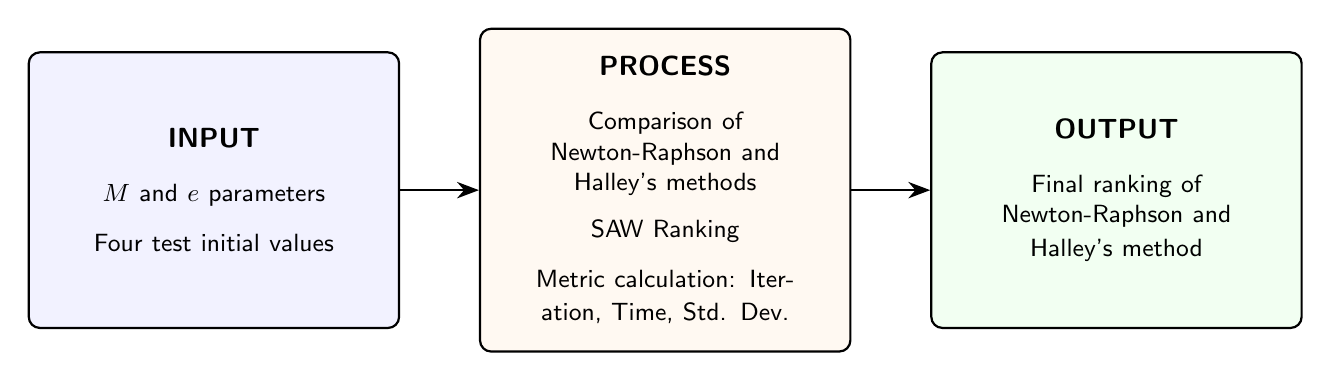
\begin{tikzpicture}[
        node distance=1cm,
        % Define a uniform style for all blocks
        block/.style={
            rectangle, 
            draw=black, 
            thick, 
            text width=4cm,   % Uniform width
            minimum height=3.5cm, % Uniform height for all boxes
            align=center, 
            rounded corners,
            inner sep=10pt % Padding inside the boxes
        },
        arrow/.style={
            -{Stealth[scale=1.2]},
            thick
        }
    ]

    % Draw the Nodes
    \node (input) [block, fill=blue!5] {
        \textbf{INPUT}\\
        \vspace{0.3cm}
        \small
        $M$ and $e$ parameters \\
        \medskip
        Four test initial values
    };

    \node (process) [block, right=of input, fill=orange!5] {
        \textbf{PROCESS}\\
        \vspace{0.3cm}
        \small
        Comparison of Newton-Raphson and Halley's methods \\
        \medskip
        SAW Ranking \\
        \medskip
        Metric calculation: Iteration, Time, Std. Dev.
    };

    \node (output) [block, right=of process, fill=green!5] {
        \textbf{OUTPUT}\\
        \vspace{0.3cm}
        \small
        Final ranking of \\
        Newton-Raphson and \\
        Halley's method
    };

    % Draw the connecting arrows
    \draw [arrow] (input) -- (process);
    \draw [arrow] (process) -- (output);

    \end{tikzpicture}
\end{figure}

\section{Results}

Table \ref{tab:test-summary} below summarizes the parameters used in the numerical methods for each test case. The mean anomaly (M) and eccentricity remains the same 7deg and 0.999 respectively across all four test cases. Only the initial value E0 varies per case and is tested on the study. 

\begin{table}[H]
    \centering
    \caption{Experimental Test Case Parameters}
    \label{tab:test-summary}
    \vspace{2mm}
    \begin{tabular}{cccc}
        \toprule
        Test Case & $M$ (deg) & $e$ & $E_0$ \\
        \midrule
        1 & \ang{7} & 0.999 & \SI{0.122173}{rad} or \ang{7} \\
        2 & \ang{7} & 0.999 & 0.6724 \\
        3 & \ang{7} & 0.999 & 0.9744 \\
        4 & \ang{7} & 0.999 & 0.9744 \\
        \bottomrule
    \end{tabular}
\end{table}

The table \ref{tab:result_1}  below shows the results of the solutions of each method in solving for the first case where E0 = M. It can be seen that Halley's method converged the fastest with only 6 iterations and had the smallest residual of all the methods and had an average computation time of 7 $\mu$s and 0.0103 standard deviation. Lastly, Newton-Raphson converged on 44 iterations as also observed by Ozuomba (2014) with the same parameters given.

\begin{table}[H]
    \centering
    \caption{Performance Comparison for Test Case 1}
    \label{tab:result_1}
    \vspace{2mm}
    \begin{tabularx}{\textwidth}{clcccccc}
        \toprule
        Method & Root (Rad) & Iterations & Avg ($\mu$s) & Std Dev ($\mu$s) & Best ($\mu$s) & Residual Error \\
        \midrule
         Halley & 0.912288 & 6 & 7.1471 & 0.0103 & 7.1252 & $5.55 \times 10^{-17}$ \\
         Secant & 0.912288 & 7 & 4.6315 & 0.0087 & 4.6210 & $6.19 \times 10^{-14}$ \\
         Fixed Point & 0.912276 & 26 & 8.5263 & 0.0149 & 8.4946 & $4.70 \times 10^{-06}$ \\
         Newton & 0.912288 & 44 & 30.8913 & 0.4835 & 30.5227 & $4.27 \times 10^{-12}$ \\
        \bottomrule
    \end{tabularx}
\end{table}

The results of the second case is shown in Table \ref{tab:result-2} where Halley's method still outpaced the rest in terms of convergence with iteration of only 3. Newton followed with 5 iterations converging with the same residual. In terms of runtime, Fixed-point method took the longest with an average of 7 $\mu$s while Newton computed the fastest with only 3.49 $\mu$s followed closely by Halley's method of around 3.6 $\mu$s.


\begin{table}[H]
    \centering
    \caption{Performance Comparison for Test Case 2}
    \label{tab:result-2}
    \vspace{2mm}
    \begin{tabularx}{\textwidth}{clcccccc}
        \toprule
        Method & Root (Rad) & Iterations & Avg ($\mu$s) & Std Dev ($\mu$s) & Best ($\mu$s) & Residual Error \\
        \midrule
         Halley & 0.912288 & 6 & 7.1471 & 0.0103 & 7.1252 & $5.55 \times 10^{-17}$ \\
         Secant & 0.912288 & 7 & 4.6315 & 0.0087 & 4.6210 & $6.19 \times 10^{-14}$ \\
         Fixed Point & 0.912276 & 26 & 8.5263 & 0.0149 & 8.4946 & $4.70 \times 10^{-06}$ \\
         Newton & 0.912288 & 44 & 30.8913 & 0.4835 & 30.5227 & $4.27 \times 10^{-12}$ \\
        \bottomrule
    \end{tabularx}
\end{table}

Halley's method still converged the fastest still with 3 iterations and a computation time of 3.69 $\mu$s as shown in Table. Newton's method however, improved to 4 iterations in the third case while still being the fastest in computation time with just around 2.87 $\mu$s. Both Halley's and Newton-Raphson methods had the same residual error.


\begin{table}[H]
    \centering
    \caption{Performance Comparison for Test Case 3}
    \label{tab:result-3}
    \vspace{2mm}
    \begin{tabularx}{\textwidth}{clcccccc}
        \toprule
        Method & Root (Rad) & Iterations & Avg ($\mu$s) & Std Dev ($\mu$s) & Best ($\mu$s) & Residual Error \\
        \midrule
         Halley & 0.912288 & 6 & 7.1471 & 0.0103 & 7.1252 & $5.55 \times 10^{-17}$ \\
         Secant & 0.912288 & 7 & 4.6315 & 0.0087 & 4.6210 & $6.19 \times 10^{-14}$ \\
         Fixed Point & 0.912276 & 26 & 8.5263 & 0.0149 & 8.4946 & $4.70 \times 10^{-06}$ \\
         Newton & 0.912288 & 44 & 30.8913 & 0.4835 & 30.5227 & $4.27 \times 10^{-12}$ \\
        \bottomrule
    \end{tabularx}
\end{table}
For the last trial, Halley's method now converged to 2 iterations and an average runtime of 2.54 $\mu$s, followed by Newton's method of 3 iterations and an average runtime of 2.18 $\mu$s with both methods resolving to the same residual.

\begin{table}[H]
    \centering
    \caption{Performance Comparison for Test Case 4}
    \label{tab:result-4}
    \vspace{2mm}
    \begin{tabularx}{\textwidth}{clcccccc}
        \toprule
        Method & Root (Rad) & Iterations & Avg ($\mu$s) & Std Dev ($\mu$s) & Best ($\mu$s) & Residual Error \\
        \midrule
         Halley & 0.912288 & 6 & 7.1471 & 0.0103 & 7.1252 & $5.55 \times 10^{-17}$ \\
         Secant & 0.912288 & 7 & 4.6315 & 0.0087 & 4.6210 & $6.19 \times 10^{-14}$ \\
         Fixed Point & 0.912276 & 26 & 8.5263 & 0.0149 & 8.4946 & $4.70 \times 10^{-06}$ \\
         Newton & 0.912288 & 44 & 30.8913 & 0.4835 & 30.5227 & $4.27 \times 10^{-12}$ \\
        \bottomrule
    \end{tabularx}
\end{table}

For all the trials, Halley's method consistently placed first in terms of the number of iterations needed to find the root with Newton-Raphson closely following except for the first case where it struggled to find the root. However, Newton-Raphson method consistently outpaced every method in terms of the average runtime it took to find the root which is then followed closely by the Halley's method. Halley's method can be considered better than Newton-Raphson in terms of convergence, however, due to the complexity which requires the third derivative of the function, Newton-Raphson is simpler. 

To determine which numerical root finding method offers the best in terms of convergence and runtime, Simple Additive weighting was conducted and the results are shown in Table \ref{tab:saw-result-1} where for each test case, final SAW score was calculated. The saw score shown illustrates that Halley outranks 3 out of four test cases in terms of iterations, average runtime, and standard deviation while Newton-Raphson only ranks higher in test case 3.

\begin{table}[H]
    \centering
    \caption{Multi-row Comparison of SAW Scores}
    \label{tab:saw-result-1}
    \vspace{2mm}
    \begin{tabular}{c l c} % 'c' for centered columns
        \toprule
        \textbf{Test Case} & \textbf{Method} & \textbf{SAW Score} \\
        \midrule
        \multirow{2}{*}{Test 1} & Newton-Raphson & 0.8421 \\
                                & Halley's Method & 0.9567 \\
        \midrule
        \multirow{2}{*}{Test 2} & Newton-Raphson & 0.7134 \\
                                & Halley's Method & 0.8922 \\
        \midrule
        \multirow{2}{*}{Test 3} & Newton-Raphson & 0.6544 \\
                                & Halley's Method & 0.9103 \\
        \midrule
        \multirow{2}{*}{Test 4} & Newton-Raphson & 0.6544 \\
                                & Halley's Method & 0.9103 \\
        \bottomrule
    \end{tabular}
\end{table}

While Table \ref{tab:saw-result-1} shows the individual winner per test case, Table \ref{tab:saw-result-2} shows the average SAW score for all the test cases performed in the study. Halley's method has an average SAW score of 0.57 while Newton-Raphson has an average of 0.36. Therefore, with the criteria of number of iteration, average runtime, and standard deviation - Halley's method outperforms Newton-Raphson method in the test cases.

\begin{table}[H]
    \centering
    \caption{SAW Score Comparison for Numerical Methods}
    \label{tab:saw-result-2}
    \vspace{2mm}
    \begin{tabular}{l c}
        \toprule
        \textbf{Method} & \textbf{SAW Score} \\
        \midrule
        Halley's Method & 0.576096 \\
        Newton-Raphson & 0.362361 \\
        \bottomrule
    \end{tabular}
\end{table}

\section{Conclusion}

This study evaluated the performance of the Newton-Raphson and Halley's numerical methods in solving Kepler's Equation for high-eccentricity orbits ($e = 0.999$). By analyzing four distinct test cases with varying initial conditions ($E_0$), the research successfully identified the critical trade-offs between mathematical convergence and computational execution.
The findings reveal that Halley's method is the superior algorithm in terms of mathematical convergence, consistently requiring fewer iterations than the Newton-Raphson method. This was particularly evident in Case 1, where a poor initial guess ($E_0 = M$) caused the Newton-Raphson method to struggle, requiring 44 iterations to converge—a result that aligns with previous findings by Ozuomba (2014). Conversely, the Newton-Raphson method demonstrated higher computational efficiency in cases with better initial approximations, consistently achieving faster average runtimes (as low as 2.18 $\mu$s) due to its lower algorithmic complexity.
However, the Simple Additive Weighting (SAW) analysis, which integrated iteration count, average runtime, and stability (standard deviation), provided a holistic ranking that favored Halley's method. With an average SAW score of 0.57 against Newton-Raphson's 0.36, Halley's method proved to be the more robust and reliable solver. While Newton-Raphson is faster in "steady-state" scenarios, Halley's method's ability to maintain rapid convergence under difficult initial conditions makes it the more effective choice for the high-stress numerical environments typical of satellite navigation.

\section{Recommendations}

Based on the results and conclusions of this study, the following are recommended for future research and practical application:
\begin{enumerate}
    \item \textbf{Low level implementations}. The python programming language was used in the study which is a high-level language. Future research should implement these algorithms in low-level languages such as C++ or Assembly. This would allow for a better assessment for both methods. 
    \item \textbf{Memory as metric.} It is recommended to also evaluate the memory as a potential criteria to see how much memory each numerical method consumes which may be crucial in some low-resource devices.
    \item \textbf{Expansion of Decision Criteria} It is recommended to change the weights of the SAW criteria based on specific profiles. For example, a higher weight in average runtime may be needed for comparison in minimizing power consumption of these numerical methods.


\end{enumerate}


\newpage
\section{References}
\printbibliography[heading=none]
\newpage

\appendix
\section{Appendix}


\end{document}
